\chapter{Problematyka zagadnienia}
\label{ch:problematyka}

%---------------------------------------------------------------------------
\section{Charakterystyka choroby Parkinsona}
\label{sec:charakterystykaPD}

Choroba Parkinsona (PD) to zwyrodnieniowe schorzenie mózgu, które wiąże się z objawami ruchowymi, takimi jak spowolnienie ruchowe,
drżenie, sztywność oraz zaburzenia chodu i równowagi.
Ponadto, to schorzenie może prowadzić do różnorodnych powikłań niemotorycznych, obejmujących zaburzenia poznawcze, stany psychiczne,
trudności ze snem oraz dolegliwości sensoryczne, w tym ból.
Początkowe objawy często rozwijają się stopniowo, nasilając się w miarę upływu czasu.
Postęp choroby prowadzi do znacznego stopnia niepełnosprawności, co może wymagać wsparcia i opieki.
U wielu osób zdiagnozowanych z chorobą Parkinsona występują także zmiany w sferze psychicznej i behawioralnej, takie jak
trudności ze snem, depresja, problemy z pamięcią oraz uczucie przewlekłego zmęczenia.

\begin{figure}[htbp]
	\centering
	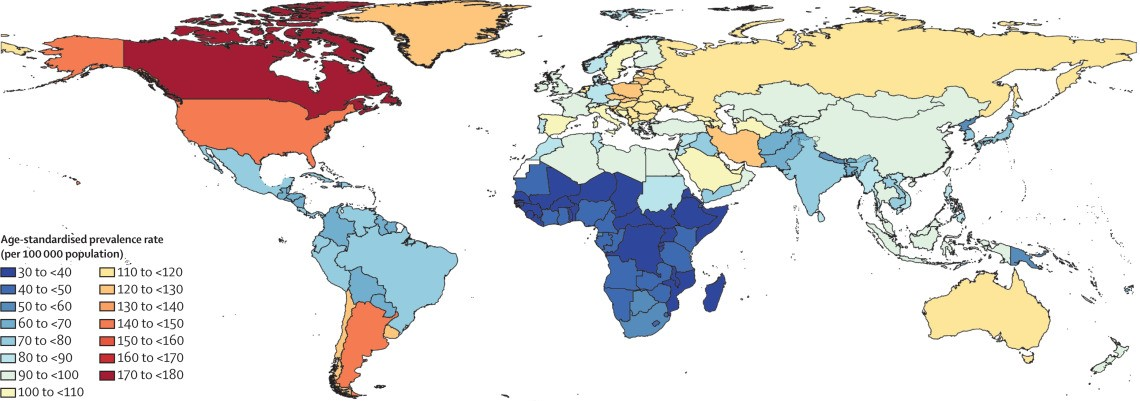
\includegraphics[width=0.9\textwidth]{./img/map}
	\caption{Choroba Parkinsona na świecie \cite{global_PD}}
    \label{fig:PD_map}
\end{figure}

Zgodnie z danymi przedstawionymi w raporcie Światowej Organizacji Zdrowia \cite{WHO}, choroba Parkinsona (PD) stanowi obecnie narastający problem na skalę światową. Zarówno wskaźniki niepełnosprawności, jak i zgony związane z tą chorobą rosną szybciej niż w przypadku innych zaburzeń neurologicznych.

W ciągu ostatnich 25 lat zaobserwowano podwojenie częstości występowania PD na całym świecie.
Globalne szacunki na rok 2019 wskazują, że liczba osób cierpiących na PD przekroczyła 8,5 miliona.
Co więcej, analizy obrazują, że w 2019 roku PD spowodowała aż 5,8 miliona lat życia z niepełnosprawnością, co oznacza wzrost
o imponujące 81\% w porównaniu z danymi z roku 2000.
Jednocześnie liczba zgonów związanych z tą chorobą wyniosła 329 000, co stanowi wzrost o ponad 100\% w porównaniu z rokiem 2000 \cite{global_PD}.

PD jest istotną sprawą dotyczącą zdrowia publicznego, ponieważ jej częstotliwość występowania związana jest ze zjawiskiem starzejącego się społeczeństwa.
Razem z innymi chorobami neurodegeneracyjnymi, takimi jak choroba Alzheimera, PD ma szanse stać się drugą zaraz za nowotorami przyczyną zgonów do 20240 roku (WHO).

W Polsce z chorobą Parkinsona zmaga się około 100 tys. pacjentów, z czego około 20\% jest już w stadium zaawansowanym
według informacji przekazywanych przez Fundację Chorób Mózgu.
Ponadto co roku w naszym kraju wykrywanych jest ok. 8 tys. nowych zachorowań.
Nowe zachorowania nadal skorelowane są z wiekiem, średnia wieku chorych wynosi 60 lat, niestety wzrasta odsetek chorych wśród osób młodych (nawet w wieku 20 lat).

Przyczyna PD nie jest znana, ale uważa się, że powstaje w wyniku złożonej interakcji pomiędzy czynnikami genetycznymi i
narażeniem na czynniki środowiskowe, takie jak pestycydy, rozpuszczalniki i zanieczyszczenia powietrza.
Niektóre przypadki PD wydają się być dziedziczne, a kilka przypadków można przypisać określonym wariantom genetycznym.
Chociaż uważa się, że genetyka odgrywa rolę w chorobie Parkinsona, w większości przypadków choroba nie występuje rodzinnie\cite{National_Institute_on_Aging_2022}.

\begin{figure}[htbp]
	\centering
	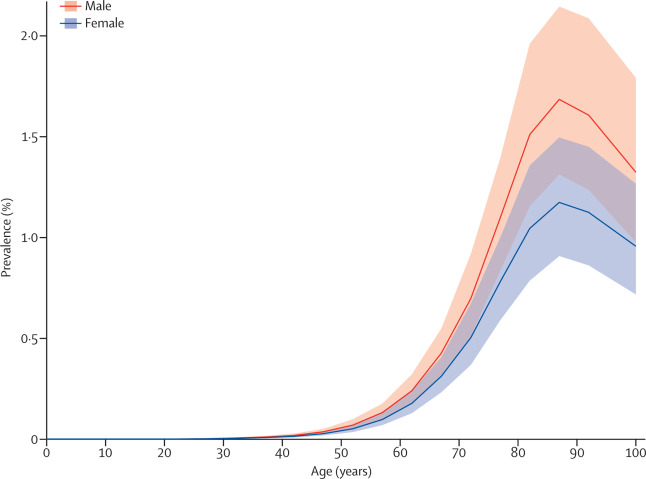
\includegraphics[width=0.6\textwidth]{./img/PD_prevalence}
	\caption{Rozpowszechnienie choroby Parkinsona w zależności od wieku \cite{global_PD}}
    \label{fig:PD_prevalance}
\end{figure}

Chociaż każdy może być narażony na ryzyko rozwoju choroby Parkinsona to obserwuje się, że choroba Parkinsona występuje częściej u mężczyzn niż u kobiet,
a wiek stanowi kluczowy element wpływający na ryzyko zachorowania, co można zobaczyć na Rys.\ref{fig:PD_prevalance}.
Statystyki pokazują, że ryzyko zachorowania rośnie wraz z wiekiem, chociaż choroba może dotyczyć także młodszych osób.
U większości osób z PD po raz pierwszy choroba rozwija się po 60 roku życia, około 5\% do 10\% doświadcza jej początku przed 50 rokiem życia.
Postacie choroby Parkinsona o wczesnym początku są często, choć nie zawsze, dziedziczne i niektóre formy zostały powiązane z
określonymi zmianami w genach \cite{National_Institute_on_Aging_2022}.

%---------------------------------------------------------------------------

\subsection{Objawy choroby}
\label{subsec:objawy}

Najbardziej widoczne oznaki i objawy choroby Parkinsona pojawiają się, gdy komórki nerwowe w zwojach podstawy mózgu,
obszarze mózgu kontrolującym ruch, ulegają uszkodzeniu i/lub obumierają.
Zwykle te komórki nerwowe lub neurony wytwarzają dopaminę.
Kiedy neurony obumierają lub ulegają uszkodzeniu, wytwarzają mniej dopaminy, co powoduje problemy z poruszaniem się
związane z chorobą.
Na ten moment nie wiadomo co powoduje śmierć neuronów.
Zanikają również zakończenia nerwowe, które wytwarzają norepinefrynę, główny przekaźnik chemiczny
współczulnego układu nerwowego, który kontroluje wiele funkcji organizmu, takich jak tętno i ciśnienie krwi.
Utrata norepinefryny może pomóc wyjaśnić niektóre cechy choroby Parkinsona związane z brakiem ruchu, takie jak zmęczenie,
nieregularne ciśnienie krwi, zmniejszony ruch pokarmu w przewodzie pokarmowym i nagły spadek ciśnienia krwi, gdy osoba wstaje z pozycji siedzącej lub leżącej.

\vspace{0.5cm}
Do czterech głównych objawów choroby Parkinsona zalicza się:
\begin{itemize}[itemsep=0.05pt]
	\item Drżenie rąk, ramion, nóg, szczęki lub głowy
	\item Sztywność mięśni, gdy mięśnie pozostają skurczone przez długi czas
	\item Powolność ruchu
	\item Zaburzenia równowagi i koordynacji, czasami prowadzące do upadków
\end{itemize}

\vspace{0.15cm}
Pozostałe objawy mogą obejmować:
\begin{itemize}[itemsep=0.05pt]
	\item Depresja i inne zmiany emocjonalne
	\item Trudności w połykaniu, żuciu i mówieniu
	\item Problemy z układem moczowym lub zaparcia
	\item Problemy skórne
\end{itemize}


Objawy choroby Parkinsona oraz tempo jej postępu mogą znacząco różnić się wśród poszczególnych osób.
Na wczesnym etapie choroby objawy są subtelne i kształtują się stopniowo.
Często zaczynają się od jednej strony ciała lub nawet jednej kończyny.
W miarę jak choroba rozwija się, dotyka ona ostatecznie obu stron, jednak niekiedy objawy mogą być bardziej intensywne po jednej stronie niż po drugiej.
Niektórzy pacjenci z chorobą Parkinsona doświadczają pewnych zwiastunów przed wystąpieniem charakterystycznych cech, takich jak sztywność czy drżenie.
Mogą to być trudności ze snem, problemy z wypróżnianiem, utrata węchu czy także zespół niespokojnych nóg.
Warto jednak zaznaczyć, że niektóre z wymienionych objawów mogą również występować w procesie naturalnego starzenia się \cite{National_Institute_on_Aging_2022}.


Chociaż tempo postępu choroby Parkinsona zazwyczaj jest powolne, w końcu ma to wpływ na codzienne funkcjonowanie osoby dotkniętej tą dolegliwością.
Wykonywanie zwykłych czynności, takich jak praca, prowadzenie domu czy uczestnictwo w spotkaniach towarzyskich z przyjaciółmi, może stawać się wyzwaniem.

%---------------------------------------------------------------------------

\subsection{Terapia osób chorych}
\label{subsec:terapia}
Obecnie brak jest kuracji na chorobę Parkinsona, dlatego terapia skupia się na przywracaniu pacjentom zdolności funkcjonowania
lub, w przypadkach zaawansowanych, na poprawie jakości życia.
Zgodnie z aktualnym standardem medycznym, w terapii wykorzystuje się różnorodne metody, w tym leczenie farmakologiczne, głęboką stymulację mózgu oraz rehabilitację \cite{National_Institute_on_Aging_2022}.

Leczenie farmakologiczne choroby Parkinsona opiera się na zwiększeniu poziomu dopaminy w mózgu, co wpływa na kontrolę objawów
ruchowych i niezwiązanych z ruchem. Główną terapią jest lewodopa, która jest przetwarzana przez komórki nerwowe w dopaminę.
Leczenie lewodopą często łączy się z karbidopą, która zmniejsza skutki uboczne i ilość potrzebnej lewodopy.
Stosuje się też inne terapie farmakologiczne o różnych zasadach działania m.in. pobudzające produkcję dopaminy,
zwiększające ilość dopaminy poprzez spowolnienie jej rozkładu, redukujące ruchy mimowolne czy zmniejszające drżenie i sztywność mięśni.

W przypadku pacjentów, u których leczenie farmakologiczne nie przynosi oczekiwanych efektów, może być rozważana Głęboka Stymulacja Mózgu (DBS).
W tym procederze chirurgicznym lekarz implantuje elektrody w określone obszary mózgu, łącząc je z małym urządzeniem elektrycznym umieszczonym w klatce piersiowej.
Poprzez bezbolesne stymulowanie konkretnych obszarów mózgu kontrolujących ruch, DBS może pomóc w zmniejszeniu wielu objawów związanych z ruchem,
takich jak drżenie, spowolnienie ruchu i sztywność.

Kluczową rolę w leczeniu odgrywa rehabilitacja neurologiczna, rozpoczynając się już od momentu postawienia diagnozy.
Jej wsparcie jest nieocenione w łagodzeniu zaburzeń chodu, głosu, drżenia, sztywności oraz pogorszenia funkcji umysłowych.
Wśród różnorodnych terapii, znajdują się między innymi:
\begin{itemize}[itemsep=0.1pt]
	\item Zbilansowana Dieta: Odpowiednio zbilansowana dieta odgrywa istotną rolę we wspieraniu ogólnego samopoczucia pacjenta.
	\item Ćwiczenia Fizyczne: Regularne ćwiczenia wzmacniają mięśnie, poprawiają równowagę, elastyczność i koordynację, co może znacząco wpłynąć na jakość życia.
	\item Masaż Terapeutyczny: Masaż terapeutyczny pomaga w redukcji napięcia mięśniowego oraz przynosi ulgę w objawach.
	\item Joga i Tai Chi: Zajęcia z jogi i tai chi wspomagają rozciąganie i elastyczność ciała, co może korzystnie wpłynąć na zdolność ruchową.
	\item Rehabilitacja Foniczna: Specjalistyczna terapia foniczna pomaga w eliminowaniu trudności w mówieniu.
	\item Psychoterapia: Psychoterapia odgrywa istotną rolę w poprawie jakości życia, umożliwiając pacjentom pełne cieszenie się życiem pomimo choroby.
\end{itemize}

Rehabilitacja neurologiczna stanowi nieodzowny element kompleksowego podejścia do zarządzania chorobą Parkinsona, pomagając pacjentom w utrzymaniu jak najwyższej jakości życia.

%---------------------------------------------------------------------------

\section{Metody diagnozowania i monitorowania}
\label{subsec:diagnostyka}

Diagnostyką choroby Parkinsona zajmują się neurolodzy i geriatrzy.
Jej rozwój jest długotrwały, a w początkowych latach klinicznie niemal niewidoczny, co utrudnia wczesne rozpoznanie.
Subtelne objawy często są uważane za skutek starzenia się lub błędnie diagnozowane jako inne zaburzenia neurologiczne.
Kluczowym elementem w tym stadium jest dokładny wywiad, badanie fizykalne oraz identyfikacja objawów przez lekarza.
Następnie diagnoza jest rozwijana poprzez badania laboratoryjne  oraz obrazowe.
Niestety, wyniki tych badań rzadko potwierdzają diagnozę od razu.

Początkowo pacjent zwykle konsultuje się z lekarzem pierwszego kontaktu, który powinien dokonać wstępnej diagnozy i skierować do neurologa.
W tej fazie diagnozy przeprowadza się szczegółowy wywiad, uwzględniający rodzaj, nasilenie oraz okres występowania objawów, a także
obecność chorób neurozwyrodnieniowych w rodzinie.
Neurolog przeprowadza kompleksowe badanie neurologiczne, identyfikując symptomy takie jak sztywność mięśni, ograniczenia w
ruchu (spowolnienie, trudności w poruszaniu się), drżenia spoczynkowe (np. w głowie, palcach rąk) oraz zaburzenia postawy i równowagi
(zgarbienie, niestabilność, upadki). Kolejne badania są wykonywane w celu potwierdzenia lub wykluczenia diagnozy \cite{diagnostyka_Sitek, Loscalzo_2022}.

\renewcommand{\labelenumi}{\alph{enumi})}
\begin{enumerate}
	\item Badania laboratoryjne
	\item[] Obecnie brak specyficznych badań laboratoryjnych krwi, które potwierdzałyby diagnozę choroby Parkinsona.
Niemniej jednak, takie badania są użyteczne w wykluczaniu innych chorób o podobnym przebiegu.
Wykonuje się podstawowe badania, takie jak morfologia krwi, elektrolity, poziom glukozy, TSH, próby wątrobowe, mocznik, kreatynina oraz poziom witaminy B12.

	\item Badania obrazowe
	\item[] Badania obrazowe głowy są przeprowadzane w celu wykluczenia innych chorób o podobnych objawach.
Pomimo że nie są one szczególnie pomocne w diagnozowaniu choroby Parkinsona, odgrywają ważną rolę w diagnostyce różnicowej.
Do tych badań zalicza się tomografię komputerową, ultrasonografię mózgu (USG) oraz rezonans magnetyczny głowy (MRI). Chociaż badania te nie potwierdzają choroby Parkinsona, mogą ujawnić obecność guzów mózgu czy wodogłowia.
Międzynarodowe kryteria rozpoznania choroby Parkinsona nie nakładają obowiązku wykonywania badań obrazowych w celu potwierdzenia diagnozy.
Warto jednak wiedzieć, że dostępne są również zaawansowane techniki obrazowania, takie jak PET (pozytonowa emisyjna tomografia) oraz SPECT (tomografia emisyjna pojedynczego fotonu),które pozwalają na obserwację metabolizmu w układzie pozapiramidowym. Skan DAT (skan transportera dopaminy) jest przykładem SPECT i może być sugerowany przez specjalistę.
Mimo to, ostateczna diagnoza opiera się na objawach oraz wynikach badania neurologicznego. Większość pacjentów nie wymaga skanowania DAT.


	\item Test z lewodopą
	\item[]Test polega na podaniu pacjentowi podejrzewanemu o chorobę Parkinsona preparatu z lewodopą.
Jeśli następuje poprawa po zażyciu, istnieje wysokie prawdopodobieństwo, że pacjent rzeczywiście cierpi na chorobę Parkinsona.
W przypadku braku poprawy, konieczne może być dalsze rozszerzenie diagnostyki.

	\item Badania genetyczne
	\item[]Choroba Parkinsona może występować w rodzinach, co skłania do rozważenia diagnostyki genetycznej u pacjenta i jego krewnych.
Badania te są wskazane, gdy lekarz podejrzewa dziedziczne występowanie choroby.
Obecnie zidentyfikowano 12 mutacji genów, które mogą wpływać na ryzyko zachorowania na chorobę Parkinsona.
Należy jednak zaznaczyć, że badania genetyczne są kosztowne.
Proszę, daj znać, czy taka wersja Ci odpowiada, czy może potrzebujesz dalszych zmian.


	\item Badania węchu
	\item[]Większość osób z chorobą Parkinsona (90\%) doświadcza zaburzeń węchu, manifestujących się hiposomią (osłabienie węchu), także we wczesnym stadium choroby.
Jednak nie obserwuje się tych zaburzeń w przypadku zaniku wieloukładowego i postępującego porażenia nadjądrowego.

	\item Badania neuropsychologiczne i neuropsychiatryczne
	\item[]Badania te służą identyfikacji zaburzeń poznawczych i emocjonalnych u osób z podejrzeniem choroby Parkinsona.
Psycholodzy i psychiatrzy mają za zadanie diagnozować łagodne zaburzenia poznawcze, otępienie, a także zaburzenia psychotyczne, lękowe, zachowania, kontroli impulsów i depresję.
Proces diagnostyczny jest dostosowany indywidualnie do możliwości pacjenta.
\end{enumerate}

Naukowcy badają test amplifikacji nasion alfa-synukleiny, zdolny do wykrywania choroby Parkinsona przed pojawieniem się objawów.
Test identyfikuje skupiska białka alfa-synukleiny w płynie rdzeniowym, charakterystyczne dla ciał Lewy'ego w mózgu.
Badanie z 2023 roku na ponad 1000 osobach wykazało, że test trafnie rozpoznał chorobę Parkinsona w 87,7\% przypadków.
Wyniki sugerują, że ten test może zmienić podejście do diagnozy, badań i terapii choroby Parkinsona.
Planuje się przyszłe badania oraz nadzieję na mniej inwazyjne metody, takie jak próbki krwi, do przeprowadzania testu \cite{Mayo_Clinic_PD}.

Objawy przypominające chorobę Parkinsona mogą być spowodowane różnymi zaburzeniami, takimi jak zanik wieloukładowy, demencja z ciałami Lewy'ego czy postępujące porażenie nadjądrowe. Te schorzenia są z kolei diagnozowane jako parkinsonizm.

Właściwe odróżnienie między tymi chorobami jest istotne, ponieważ leczenie i podejście terapeutyczne różnią się \cite{National_Institute_on_Aging_2022}.
Badania medyczne oraz reakcja na leczenie farmakologiczne mogą pomóc w ustaleniu dokładnej przyczyny.
Ważne jest, aby uzyskać szybką i dokładną diagnozę.

Choroby o podobnym przebiegu do choroby Parkinsona obejmują m.in. postępujące porażenie nadjądrowe, zanik wieloukładowy, drżenie samoistne, choroby naczyniowe mózgu, otępienie, reumatyzm oraz inne \cite{diagnostyka_Sitek}.
Różnicowanie tych schorzeń jest kluczowe dla właściwego leczenia i zarządzania pacjentem.

Diagnostyka różnicowa choroby Parkinsona obejmuje różne formy parkinsonizmu oraz inne stany neurodegeneracyjne.
Chociaż ostateczną diagnozę można ustalić tylko na podstawie badania mózgu po zgonie, wcześniej zdefiniowane kryteria diagnostyczne pozwalają na dokonanie diagnozy klinicznej.
Przyjęcie ram czasowych (3-10 lat) dla postawienia klinicznie potwierdzonej diagnozy choroby Parkinsona opiera się na empirycznych dowodach.
Wnioski płynące z badania \cite{ROSSI202153} sugerują, że diagnoza klinicznie potwierdzonej choroby Parkinsona może zabierać od kilku miesięcy do kilku lat, zależnie od indywidualnych czynników oraz reakcji na terapię lewodopą.

Chorobę Parkinsona wykluczają także pewne kryteria. Zalicza się do nich:
\begin{itemize}[itemsep=0.5pt]
	\item Historia wielokrotnych urazów głowy,
	\item Przebyte zapalenie mózgu,
	\item Podobne objawy u więcej niż jednej osoby w rodzinie,
	\item Leczenie neuroleptykami w momencie objawów,
	\item Przebyte udary mózgu z nasilonymi objawami parkinsonowskimi,
	\item Długotrwałe ustąpienie objawów,
	\item Objawy po jednej stronie ciała przy chorobie trwającej ponad 3 lata.
\end{itemize}


Pomocnym narzędziem w dianostyce są szeroko stosowane skale oceny choroby Parkinsona.
Stanowią istotne narzędzie w monitorowaniu stanu pacjentów oraz ocenie postępów choroby.
Te strukturalne i skwantyfikowane metody pomagają lekarzom i opiekunom ocenić stopień nasilenia objawów ruchowych,
jak również wpływ choroby na codzienne funkcjonowanie pacjenta.
Popularne skale, takie jak Skala Hoehn-Yahra, Skala UPDRS (Unified Parkinson's Disease Rating Scale) oraz Skala Schwab-England,
umożliwiają obiektywną analizę symptomów i wsparcie w podejmowaniu decyzji terapeutycznych.
Dzięki tym narzędziom możliwe jest dostosowanie leczenia do indywidualnych potrzeb pacjenta oraz śledzenie skuteczności terapii na przestrzeni czasu.


Proces diagnozowania choroby Parkinsona to zadanie wymagające czasu i precyzji.
W celu skutecznej identyfikacji i monitorowania pacjentów z tym schorzeniem, zaleca się regularne wizyty kontrolne u neurologów specjalizujących się w zaburzeniach ruchowych. Tego rodzaju wizyty pozwalają na bieżące ocenianie stanu zdrowia oraz objawów, umożliwiając dokładną diagnozę choroby Parkinsona.

Obecnie proces diagnozy jest wyjątkowo złożony i wieloetapowy.
W odpowiedzi na te wyzwania, naukowcy koncentrują się na opracowaniu bardziej efektywnych narzędzi diagnostycznych.
Poszukiwane są innowacyjne metody, które przyspieszą i usprawnią ten proces.
Rozwinięcie skuteczniejszych narzędzi diagnostycznych przyniesie korzyści nie tylko finansowe, ale także pozwoli na szybsze i trafniejsze udzielanie pomocy pacjentom cierpiącym na chorobę Parkinsona.
Poprawa diagnozy pomoże podnieść standard życia osób dotkniętych tym schorzeniem, co jest priorytetem dla społeczności medycznej i pacjentów.

W nadchodzących latach, dążenie do wypracowania bardziej efektywnych metod diagnozowania choroby Parkinsona będzie kluczowym krokiem w zapewnieniu lepszej opieki zdrowotnej i poprawie jakości życia pacjentów.

%---------------------------------------------------------------------------
%---------------------------------------------------------------------------

\section{Znaczenie głosu}
\label{sec:znaczenie_glosu}

Objawy zaburzeń mowy w chorobie Parkinsona zazwyczaj ujawniają się w średniozaawansowanym stadium, co oznacza, że przez długi okres mowa pozostaje w miarę poprawna.
Czasami trudno jest określić, czy pojawiające się zaburzenia głosu są wynikiem choroby czy naturalnego procesu starzenia się organizmu.
Starzenie się wpływa na fizjologiczne upośledzenie słuchu, co może prowadzić do zmiany brzmienia głosu - staje się on osłabiony i może zacząć
drżeć, a zakres jego tonacji może się zawężać.

\vspace{0.5cm}
Objawy zaburzeń głosu i mowy w chorobie Parkinsona nie są oczywiste i łatwe do zauważenia dla osób niebędących specjalistami.
Rozumienie mowy zwykle pozostaje nienaruszone.
W trakcie mowy spontanicznej pacjenci zaczynają jednak przekazywać mniej informacji i mogą napotykać trudności w konstruowaniu pełnych zdań.
Te trudności niekoniecznie są związane z utratą zasobu słów, a raczej wynikają z nieprawidłowego użycia słów.
Objawy, które wskazują na ich chorobowe podłoże obejmują między innymi \cite{Szurek_2018, Kuryłowicz_2019}:
\begin{itemize}[itemsep=0.5pt]
	\item Pogłębione wyciszenie głosu,
	\item Powolną, monotonną i przerywaną mowę,
	\item Zubożenie mimiki,
	\item Nadmierne ślinienie się,
	\item Niewyraźną i zamazaną artykulację,
	\item Brak ruchów mimicznych, maskowatą twarz,
	\item Skrócony czas fonacji
	\item Chuchający i tremolujący głos
	\item Spłaszczona barwa i obniżone natężenie
	\item Niewłaściwą koordynację mięśni nasady, które mogą być zwiotczałe lub zbyt napięte,
	\item Czasami przyspieszenie tempa wypowiedzi w jej końcowej fazie, co może utrudnić zrozumienie pacjenta.
\end{itemize}

Objawy te pojawiają się w stadium średniozaawansowanym choroby, rzeczywiście są już na tyle wyraźne, że mogą być zauważone
słuchowo przez specjalistów.
Niemniej jednak badania wskazują, że istnieją subtelne zmiany w głosie, które pojawiają się jeszcze wcześniej w fazie przedobjawowej \cite{2023_PD_voice}.

W 2000 roku przeprowadzono badanie akustyczne i percepcyjne cech głosu pacjentów z chorobą Parkinsona w zależności od
ciężkości choroby \cite{https://doi.org/10.1080/136828200410654}.
Nagrania głosowe składały się z przedłużonej samogłoski /a/, śpiewu gamy oraz 1-minutowego monologu.
Głosy pacjentów z PD zarówno we wczesnym, jak i późniejszym stadium charakteryzowały się percepcyjnie ograniczoną
zmiennością tonu i głośności, oddychaniem, chropowatością i zmniejszoną głośnością.
Wysokie poziomy tonu modalnego charakteryzowały również głosy mężczyzn zarówno we wczesnych, jak i późniejszych stadiach choroby Parkinsona.
Pod względem akustycznym głosy obu grup pacjentów z PD wykazywały niższe poziomy średniego natężenia i zmniejszone
maksymalne zakresy częstotliwości fonacyjnej w porównaniu z danymi normatywnymi.
Wyniki badań sugerowały również, że głosy pacjentów z PD charakteryzowały się nadmiernym drganiem, wysoką częstotliwością
podstawową w przypadku mężczyzn i zmniejszoną zmiennością częstotliwości podstawowej w przypadku kobiet.
Podczas gdy kilka z tych cech głosu nie wydawało się pogarszać wraz z postępem choroby (tj. szorstkość, wysoki ton modalny
i podstawowa częstotliwość mówienia u mężczyzn, podstawowa zmienność częstotliwości u kobiet, niska intensywność i drżenie),
oddech, monotonność i jednogłośność, niska głośność i zmniejszony maksymalny zakres częstotliwości fonacyjnej były gorsze w
późniejszych stadiach PD. Drżenie było jedyną cechą głosu, która była kojarzona tylko z PD w późniejszym stadium.

W kolejnym badaniu dowiedziono \cite{GAMBOA1997314}, że w porównaniu z grupą kontrolną pacjenci z PD wykazywali wyższy jitter,
niższy stosunek harmonicznych do szumów (H/N), mniejszą zmienność częstotliwości i intensywności zdania oraz niższy zakres
fonacyjny oraz wyższą częstotliwość obecności głosu o niskim natężeniu, jednotonowości i zatrzymania głosu.
Wydaje się, że na te cechy nie ma wpływu czas trwania i ciężkość choroby.

Choroba Parkinsona jest wynikiem zaburzonej funkcji układu nerwowego, a jej objawy mogą obejmować różne części ciała.
To zagadnienie od dłuższego czasu przyciąga uwagę grup badawczych.
Na całym świecie prowadzone są badania nad wykorzystaniem analizy mowy do wykrywania różnych patologii i schorzeń związanych z narządem głosu.

Takie podejście pozwala na wykrycie problemów, takich jak ostre zapalenie krtani, porażenie nerwu krtaniowego wstecznego oraz dysfonia funkcjonalna,
która często dotyka osób pracujących głosem, np. nauczycieli, bez konieczności inwazyjnych badań gardła. Warto również zaznaczyć, że nowością
jest wykorzystanie parametrów sygnału mowy do diagnozowania i monitorowania chorób neurodegeneracyjnych.

Badania naukowe wykazują, że istnieje realna perspektywa wykorzystania analizy głosu również w celach automatycznej diagnostyki oraz monitorowania choroby Parkinsona.
Głębsza wiedza i zrozumienie mechanizmu objawów tej choroby może przyczynić się do stworzenia precyzyjnego narzędzia, które znacząco ułatwi pracę lekarzy
oraz poprawi jakość życia pacjentów.
To otwiera obiecującą możliwość wczesnego wykrywania i diagnozowania choroby.

Warto zaznaczyć, że część objawów, zwłaszcza we wczesnych stadiach choroby, może nie być w pełni wykrywalna dla ludzkiego ucha, ale może być
zarejestrowana i analizowana przez komputery.
Ponadto, taka analiza może być wykorzystana do oceny stanu pacjenta oraz sugerowania odpowiednich interwencji, takich jak ewentualne zmiany w
leczeniu farmakologicznym.
W rezultacie takie innowacyjne narzędzie miałoby potencjał stać się szybkim, nieinwazyjnym wsparciem diagnostyczno-terapeutycznym,
przyczyniając się do poprawy jakości opieki nad pacjentami z chorobą Parkinsona.